\documentclass[a4paper,10pt]{article}

\usepackage{amsmath}
\usepackage{amsfonts}
\usepackage{amssymb}
\usepackage[spanish]{babel}
\usepackage[utf8]{inputenc}
\usepackage{listings}
\usepackage{verbatim}
\usepackage{graphicx}

\title{Proyecto de Simulación y Programación Declarativa: Agentes }
\date{Curso 2020-2021}

\begin{document}
\maketitle
\selectlanguage{spanish}

  \begin{itemize}
      \item Darian Dominguez Alayón C-411
    \end{itemize}

\section*{Introducci\'on}\label{sec:intro}
En este proyecto se ponen de manifiesto los contenidos aprendidos sobre los agentes, los cuales fueron vistos en la asignatura de Simulaci\'on. Un agente es un sistema computacional situado dentro de un medio ambiente, dentro del cual es capaz de realizar acciones autónomas encaminadas a lograr sus objetivos. Apoy\'andonos en este concepto, en todo el contenido que trae consigo y utilizando el lenguaje de programaci\'on Haskell, estudiado en la asignatura Programaci\'on Declarativa, se propone darle soluci\'on al siguiente problema.

\section*{Orden del problema asignado}
\subsection*{Marco general}
%-----------------------------------------------------------------------------------
  El ambiente en el cual intervienen los agentes es discreto y tiene la forma de un rect\'angulo de N x M. El ambiente es de informaci\'on completa, por tanto, todos los agentes conocen toda la informaci\'on sobre el agente. El ambiente puede variar aleatoriamente cada t unidades de tiempo. El valor de t es conocido.
  
  Las acciones que realizan los agentes ocurren por turnos. En un turno, los agentes realizan sus acciones, una sola por cada agente, y modifican el medio sin que este var\'ie a no ser que cambie por una acci\'on de los agentes. En el siguiente, el ambiente puede variar. Si es el momento de cambio del ambiente, ocurre primero el cambio natural del ambiente y luego la variaci\'on aleatoria. En una unidad de tiempo ocurren el turno del agente y el turno de cambio del ambiente.
  
  Los elementos que pueden existir en el ambiente son obst\'aculos, suciedad, ni\~nos, el corral y los agentes que son llamados Robots de Casa. A continuaci\'on se precisan las caracter\'isticas de los elementos del ambiente:\\\\
  \textbf{Obst\'aculos:} Estos ocupan una \'unica casilla en el ambiente. Ellos pueden ser movidos, empuj\'andolos, por los ni\~nos, una \'unica casilla. El Robot de Casa, sin embargo, no puede moverlo. No pueden ser movidos por ninguna de las casillas ocupadas por cualquier otro elemento del ambiente.\\\\
   \textbf{Suciedad:} La suciedad es por cada casilla del ambiente. Solo puede aparecer en casillas que previamente estuvieron vac\'ias. Esta, o aparece en el estado inicial o es creada por los ni\~nos.\\\\
   \textbf{Corral:} El corral ocupa casillas adyacentes en n\'umero igual al del total de ni\~nos presentes en el ambiente. El corral no puede moverse. En una casilla del corral solo puede coexistir un ni\~no. En una casilla del corral, que est\'e vac\'ia, puede entrar un robot. En una misma casilla del corral pueden coexistir un ni\~no y un robot solo si el robot lo carga, o si acaba de dejar al ni\~no.\\\\
   \textbf{Ni\~no:} Los ni\~nos ocupan solo una casilla. Ellos en el turno del ambiente se mueven, si es posible (si la casilla no est\'a ocupada: no tiene suciedad, no est\'a el corral, no hay un Robot de Casa), y aleatoriamente (puede que no ocurra
  movimiento), a una de las casillas adyacentes. Si esa casilla est\'a ocupada por un obst\'aculo este es empujado por el ni\~no, si en la direcci\'on hay m\'as de un obst\'aculo, entonces se desplazan todos. Si el obst\'aculo est\'a en una posici\'on donde no puede ser empujado y el ni\~no lo intenta, entonces el obst\'aculo no se mueve y el ni\~no ocupa la misma posici\'on. Los ni\~nos son los responsables de que aparezca suciedad. Si en una cuadr\'icula de 3 por 3 hay un solo ni\~no, entonces, luego de que \'el se mueva aleatoriamente, una de las casillas de la cuadr\'icula anterior que est\'e vac\'ia puede haber sido ensuciada. Si hay dos ni\~nos se pueden ensuciar hasta 3. Si hay tres ni\~nos o m\'as pueden resultar sucias hasta 6. Los ni\~nos cuando est\'an en una casilla del corral, ni se mueven ni ensucian. Si un ni~no es capturado por un Robot de Casa tampoco se mueve ni
  ensucia.\\\\
   \textbf{Robot de Casa:} El Robot de Casa se encarga de limpiar y de controlar a los ni\~nos. El Robot se mueve a una de las casillas adyacentes, las que decida. Solo se mueve una casilla si no carga un ni\~no. Si carga un ni\~no puede moverse hasta dos casillas consecutivas. Tambi\'en puede realizar las acciones de limpiar y cargar ni\~nos. Si se mueve a una casilla con suciedad, en el pr\'oximo turno puede decidir limpiar o moverse. Si se mueve a una casilla donde est\'a un ni\~no, inmediatamente lo carga. En ese momento, coexisten en la casilla Robot y ni\~no. Si se mueve a una casilla del corral que est\'a vac\'ia, y carga un ni\~no, puede decidir si lo deja esta casilla o se sigue moviendo. El Robot puede dejar al ni\~no que carga en cualquier casilla. En ese momento cesa el movimiento del Robot en el turno, y coexisten hasta el pr\'oximo turno, en la misma casilla, Robot y ni\~no.\\
  
  El objetivo del Robot de Casa es mantener la casa limpia. Se considera la casa limpia si el 60\% de las casillas vac\'ias no est\'an sucias.\\

 \section*{Principales Ideas seguidas para la solución del problema}
\begin{itemize}
	\item En la orden del problema se presenta un ambiente discreto lo que significa que existe un número fijo y finito de percepciones y acciones que lo pueden modificar.
	
	\item En el ambiente, el agente tiene toda la informaci\'on sobre el estado actual y puede tormar decisiones en correspondencia a la percepci\'on que crea que es mejor seguir. Debido a la aleatoriedad del ambiente cada cierto tiempo t, el agente no podr\'a tomar decisiones pensando en el futuro. 
	
	\item El ambiente es din\'amico, pues este var\'ia cada cierto intervalo de tiempo t y dichos cambios no est\'an en control del agente. Los principales responsables de esto son los ni\~nos los cuales pueden moverse hacia una casilla adyacente, dejar suciedad en alguna casilla o empujar obst\'aculos. Los responsables de limpiar y controlar a los ni\~nos son los robots (agentes).
	
	\item Los agentes pueden realizar las acciones de cargar ni\~nos, limpiar suciedad, moverse a casillas adyacentes sin ni\~no cargado, moverse a casillas adyacentes uno o dos pasos con ni\~no cargado y dejar un ni\~no en cualquier casilla posible a excepci\'on de una con suciedad.
	
	\item Los agentes pueden moverse a una casilla vacía, con corral vacío o con suciedad. También pueden moverse a casillas que contengan niños, si el agente no está cargando uno. No se permite que un agente pueda limpiar con un niño en la mano.
	
	\item Como percepciones del ambiente del agente podemos destacar el camino al ni\~no m\'as cercano, al corral m\'as cercano, a la casilla sucia m\'as cercana y el por ciento de limpieza del ambiente.
	
	\item Tenemos dos estados para nuestros agentes. Estos pueden estar sin cargar ni\~nos o cargando ni\~nos.
	
	\item Nuestro agente tiene varias funcionalidades como son limpiar las casillas sucias, llevar a los ni\~nos al corral o en caso de no ser posible ninguna de estas entonces moverse aleatoriamente. El robot antes de realizar una acci\'on analiza el ambiente:
		\begin{itemize}
			\item Si el por ciento de casillas vac\'ias que no est\'an sucias es menor que 75 entonces el robot limpiar\'a las casillas que est\'en sucias hasta que el por ciento dicho anteriormente vuelva a estar por encima de 75.
			
			\item Si el por ciento de casillas vac\'ias que no est\'an sucias es mayor que 75 entonces el robot tratar\'a de llevar al ni\~no m\'as cercano al corral m\'as cercano.
			
			\item Si en un momento cualquiera el robot no tiene que buscar ni\~nos ni limpiar las casillas sucias entonces se mover\'a con un comportamiento random para alguna de las casillas adyacentes a \'el. 
		\end{itemize} 
		
\end{itemize}


%-----------------------------------------------------------------------------------


%-----------------------------------------------------------------------------------
\section*{Modelos de Agentes considerados (por cada agente se deben presentar dos modelos diferentes)}
Como ya se mencion\'o anteriormente el ambiente del problema es din\'amico por lo que cada cierto tiempo t el ambiente va a cambiar. Los principales responsables de esto son los ni\~nos que pueden moverse a una casilla adyacente, empujar obst\'aculos y ensuciar casillas. Tambi\'en los robots al ejecutar sus acciones cambian el ambiente. Debido a este dinamismo no podemos considerar que nuestro agente sea puramente pro-activo, pues si el ambiente cambia y las precondiciones se vuelven falsas durante el proceso, entonces el comportamiento del procedimiento se indefine o simplemente falla. En la orientaci\'on del problema tambi\'en se plantea que el agente conoce toda la informaci\'on del ambiente, por lo que puede tomar las decisiones en el momento actual del ambiente. Gracias a esto el agente es capaz de percibir los cambios en el ambiente y reaccionar de modo oportuno a los mismos
con el fin de alcanzar sus objetivos, por lo que podemos decir que el agente es reactivo. No queremos un agente puramente reactivo para que el robot no est\'e reaccionando constantemente y pueda enfocarse en un objetivo un determinado tiempo hasta lograr cumplirlo. Por tanto nuestro robot se basa en una uni\'on entre agente pro-activo y reactivo. 

%-----------------------------------------------------------------------------------
 \section*{Ideas seguidas para la implementación}

Para la implementaci\'on nos basamos en todo el razonamiento anteriormente explicado. A continuaci\'on explicaremos el c\'odigo el cual aparece en la carpeta code:

\textbf{Main.hs: } Este es el archivo principal de la aplicaci\'on. Lo primero que hace es recibir los valores requeridos por el problema como son: n\'umero de casillas con obst\'aculos, n\'umero de casillas sucias, n\'umero de casillas con ni\~nos, n\'umero de robots, tiempo que demora en cambiar el ambiente, n\'umero de turnos que va a demorar la simulaci\'on y cantidad de simulaciones.
A continuaci\'on lo que se hace es crear las listas de dichos elementos con posiciones aleatorias en el ambiente. Estas listas son usadas en la funci\'on de simulaci\'on, la cual va a ser la encargada de controlar todo el proceso. Esta funci\'on se ejecutar\'a hasta que se alcancen los turnos que se pasaron en la entrada y una vez hecho esto se devolver\'a si el ambiente qued\'o limpio o sucio (el l\'imite es 60 \%), el por ciento de limpieza alcanzado y si qued\'o alg\'un ni\~no libre (que no est\'a ni en el corral ni lo carga un robot) o no. Recordar que en un turno ocurre una acci\'on de cada agente. Si el m\'odulo de la cantidad de turnos por la que va corriendo el programa con respecto al tiempo que demora en cambiar el ambiente es igual a 0, entonces este cambia. De lo contrario el agente i-\'esimo ejecutar\'a la acci\'on que crea que es la correcta. 
Una vez terminado lo anterior para cada simulaci\'on se devolver\'a un por ciento promedio de limpieza del ambiente y si este por ciento representa que qued\'o limpio o sucio.
Destacar que cada vez que se ejecute la aplicaci\'on los resultados se guardar\'an en \textit{output.txt} por si se desean consultar posteriormente\\

En la carpeta \textit{Modules} aparecen los siguientes m\'odulos en los cuales se apoya la aplicaci\'on:

\textbf{Elements.hs: } Este m\'odulo contiene al tipo Element el cual tiene un nombre \textit{name} y una posici\'on \textit{position} para ubicar los elementos. Este m\'odulo contiene todas las funciones relacionadas con los elementos como son: \textit{create\_element}, \textit{move\_element}, etc.

\textbf{Environment.hs: } M\'odulo que se encarga de gestionar todo lo que tiene que ver con el ambiente como crear las listas de los elementos, mover los elementos, pintar y mostrar el ambiente en consola y otras funcionalidades que son importantes en el ambiente.

\textbf{Robots.hs: } Como su propio nombre indica es para hacer todo lo relacionado con los robots (agentes). Aqu\'i podemos ver todas las acciones que realiza el robot: cargar ni\~no, llevar ni\~no al corral, limpiar las casillas sucias, etc. Tambi\'en est\'a implentado el \textit{robot\_random} que se ejecutar\'a cuando el robot no tenga opciones de limpiar ni de cargar ni\~nos. 

\textbf{Utils.hs: } Aqu\'i tenemos funciones que usamos en varios lugares del c\'odigo permitiendo as\'i la refactorizaci\'on. Por ejemplo aqu\'i tenemos las funciones que tienen que ver con el random, las cuales son primordiales en el proyecto.    

 \section*{Consideraciones obtenidas a partir de la ejecución de las simulaciones del problema}
Se prob\'o varias veces la aplicaci\'on con diferentes par\'ametros y en la mayor\'ia de los casos se mostr\'o un resultado positivo en cuanto a la limpieza del ambiente gracias al trabajo de los robots. A continuaci\'on presentamos dos ejemplos :


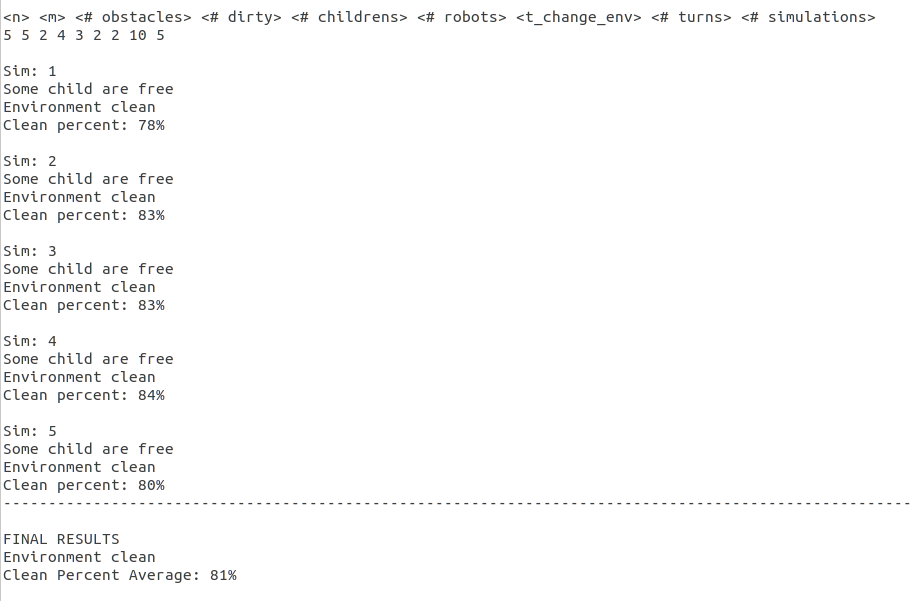
\includegraphics[width=15cm, height=10cm]{img/clean.png}\\
		
 En este ejemplo podemos ver como en las simulaciones se obtuvo un buen por ciento de limpieza lo que provoc\'o que el promedio de limpieza fuese positivo tambi\'en. Cabe destacar que en cada simulaci\'on se qued\'o al menos alg\'un ni\~no libre una vez pasado el la cantidad de turnos, que en este caso fue 10.
 
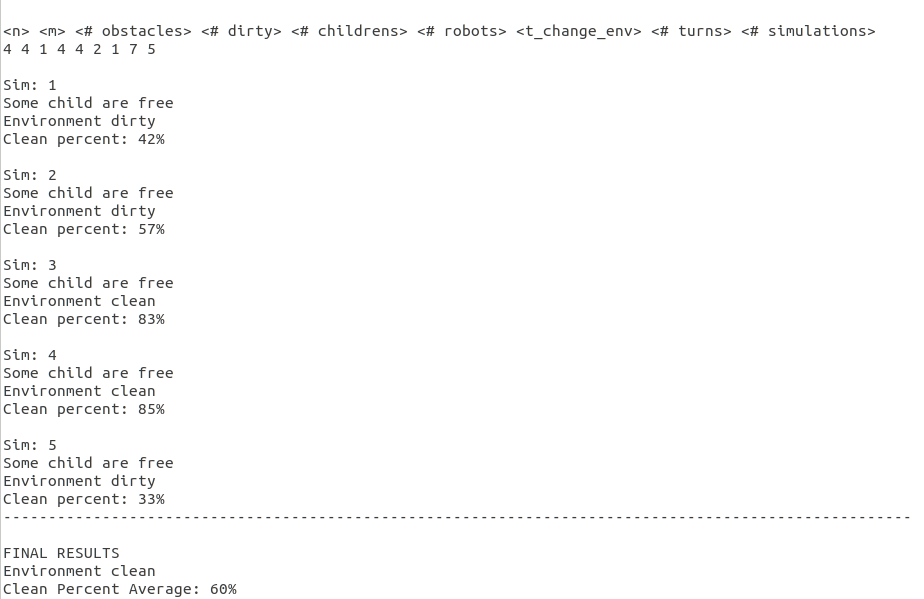
\includegraphics[width=15cm, height=10cm]{img/dirty.png}\\   

 Por otro lado podemos ver en este ejemplo que en la mayor\'ia de las simulaciones fue por debajo del 60\% por lo que el abiente en esos casos estuvo sucio. Sin embargo se observa que el promedio de limpieza fue exactamente del 60\% lo que implica que estuvo limpio, rozando el borde, el promedio de limpieza de las simulaciones. Aqu\'i tambi\'en se qued\'o al menos alg\'un ni\~no libre una vez pasados los 7 turnos.
 
\section*{Ejecuci\'on}
Para ejecutar la aplicaci\'on hay que tener instalado alg\'un compilador de haskell como \textit{ghci}, ejecutarlo en la carpeta \textit{code}, luego escribir en la consola \textit {:l Main.hs} y m\'as tarde escribir \textit{main}. Otra forma de correr la aplicaci\'on es instalar \textit{stack}, luego usando \textit{stack} instalar \textit{runhaskell} y por \'ultimo ejecutar \textit{runhaskell Main.hs} dentro de la carpeta \textit{code}. Esto funciona perfecto en Linux. En Windows puede dar problemas con el m\'odulo \textit{System.Random} por lo que se recomienda el uso de \textit{stack ghci}.
Una vez ejecutada la aplicaci\'on solo quedar\'a ingresar el n\'umero de casillas con obst\'aculos, n\'umero de casillas sucias, n\'umero de casillas con ni\~nos, n\'umero de robots, tiempo que demora en cambiar el ambiente, n\'umero de turnos que va a demorar la simulaci\'on y cantidad de simulaciones . 

\section*{Link del proyecto en GitHub}
https://github.com/Darian10/Proyecto-de-Simulacion-y-Haskell.git

%-----------------------------------------------------------------------------------
\end{document}

%===================================================================================
